\documentclass[a4paper]{article}

\usepackage[english]{babel}
\usepackage[utf8x]{inputenc}

\usepackage{amsmath}  % equations
\usepackage{cite}  % bibliograby
\usepackage{graphicx}  % images
\usepackage{pgfplots}  % plots
  \pgfplotsset{width=10cm,compat=1.9} % plots settings
  \usepgfplotslibrary{external}
  \tikzexternalize



\usepackage{hyperref}  % references
  \hypersetup{colorlinks=true,citecolor=black,filecolor=black,linkcolor=black,urlcolor=black} % references settings

\usepackage[automark]{scrpage2} % heading
  \pagestyle{scrheadings}
  \ihead[]{Handwritten character recognition in MPI} % left header
  \ohead[]{\today} % right header
  \cfoot[]{\pagemark} % footer
  \setheadsepline[122mm]{0.3mm}



\begin{document}
	\title{
	\Huge Handwritten digit recognition
	}
	
	\vspace{2cm}
	
	\author{\Large \href{mailto:stefan.niculae@my.fmi.unibuc.ro}{Stefan Niculae} \and \Large \href{mailto:ionut.ciocoiu@my.fmi.unibuc.ro}{Ionut Ciocoiu}
	\vspace{3cm}}
	
	\date{
	\large Parallel \& Concurrent Programming Lab Report \\
    \vspace{0.2cm}
	\today
	}

	\maketitle
	\setlength{\parindent}{0pt}

\vspace{5cm}
\begin{abstract}
TODO: rewrite when paper is done, talk about each section

We implement a neural network to classify handwritten digits. The training is done in parallel, using MPI. We provide a comparison for model hyper-parameters and for training time vs number of processes. It achieves great accuracy and fast training time. An interactive demo is also presented
\end{abstract}



% \newpage
% \pagestyle{plain}
% \tableofcontents



\newpage
TODO: introduction?

\section{Problem statement}
\label{sec:problem}
Given a picture of a handwritten digit, label it accordingly 0 - 9.

\section{Dataset}
\label{sec:dataset}
We demonstrate our model performance on the MNIST database, widely used dataset for training and testing in the field of machine learning. It contains 70 000 examples of labeled handwritten digits. The digits have been size-normalized and centered in a fixed-size image \cite{mnist}. 

\begin{figure}[htb]
\centering

\includegraphics[width=8cm]{images/mnist-images.png}
\caption{Sample MNIST images \cite{tf}}
\end{figure}


The images are black-and-white, with a resolution of $28 \times 28$ pixels, represented as an array of $784$ values. Each value ranges from $0$ to $1$ indicating the amount of blackness in the pixel.

\begin{figure}[htb]
\centering
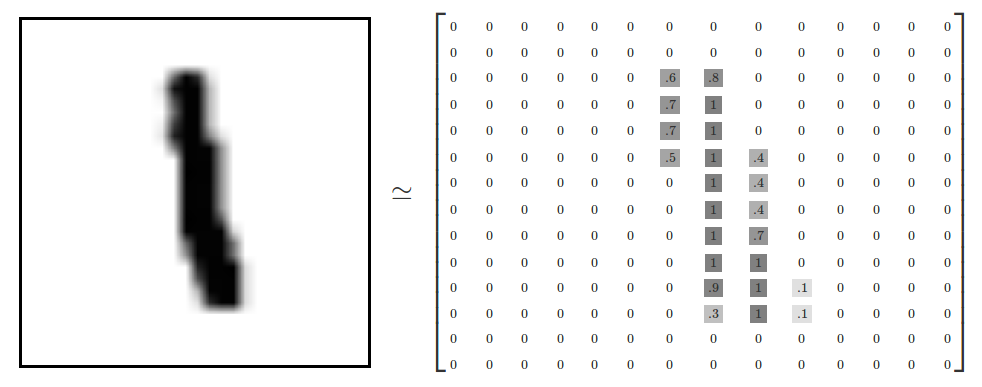
\includegraphics[width=8cm]{images/mnist-matrix.png}
\caption{Matrix representation of a digit \cite{tf}}
\end{figure}


\newpage
\section{Model}
\label{sec:model}
In order to recognize a given image, we need to model to understand the data. It needs to be able to be queried for a new instance in order to provide an interactive demo.
\\

We use a back-propagation neural network:
\begin{align*}
W^{(k)} &= W^{(k-1)} + \alpha \nabla_W^{(k-1)} \\ 
b^{(k)} &= b^{(k-1)} + \alpha \nabla_b^{(k-1)}
\end{align*}
Where $W$ is the weights matrix, $10 \times 784$ -- the number of classes( one for each digit) and the dimension of an image ($28 \times 28$). $b$ is the bias vector, $1 \times 10$, corresponding to the free element. $W^{(k)}$ denotes the weights at step $k$. $\nabla$ represents the update which must produce to improve prediction.
\\

The activation function is softmax:
$$f(x_i)=\frac{exp(x_i)}{\sum_j exp(x_j)}$$
Where $exp(x)$ represents $e^x$, Euler's constant. It \textit{normalizes} the vector, causing the greatest elements to have logarithmic relative value.
\\

The cost function is cross-entropy:
$$H(y_t, y_p)=-\sum_x y_t log(y_p)$$
Where $y_t$ is the true, correct label of an image and $y_p$ is the label predicted by the model.
\\

$L_2$ regularization is used:
$$\frac{1}{\lambda} \sum_i \sum_j W_{i,j}^2$$
Where $\lambda$ is the regularization parameter. This limits overfitting by imposing a penalty on big weights.
\\

The model uses an adaptive learning rate:
$$\eta \frac{ W^{(k)} - W^{(k-1)} } { \nabla^{(k)} - \nabla^{(k-1)} }$$
Where $\eta$ is the momentum parameter. This helps with stability in late epochs.

\begin{figure}[htb]
\centering
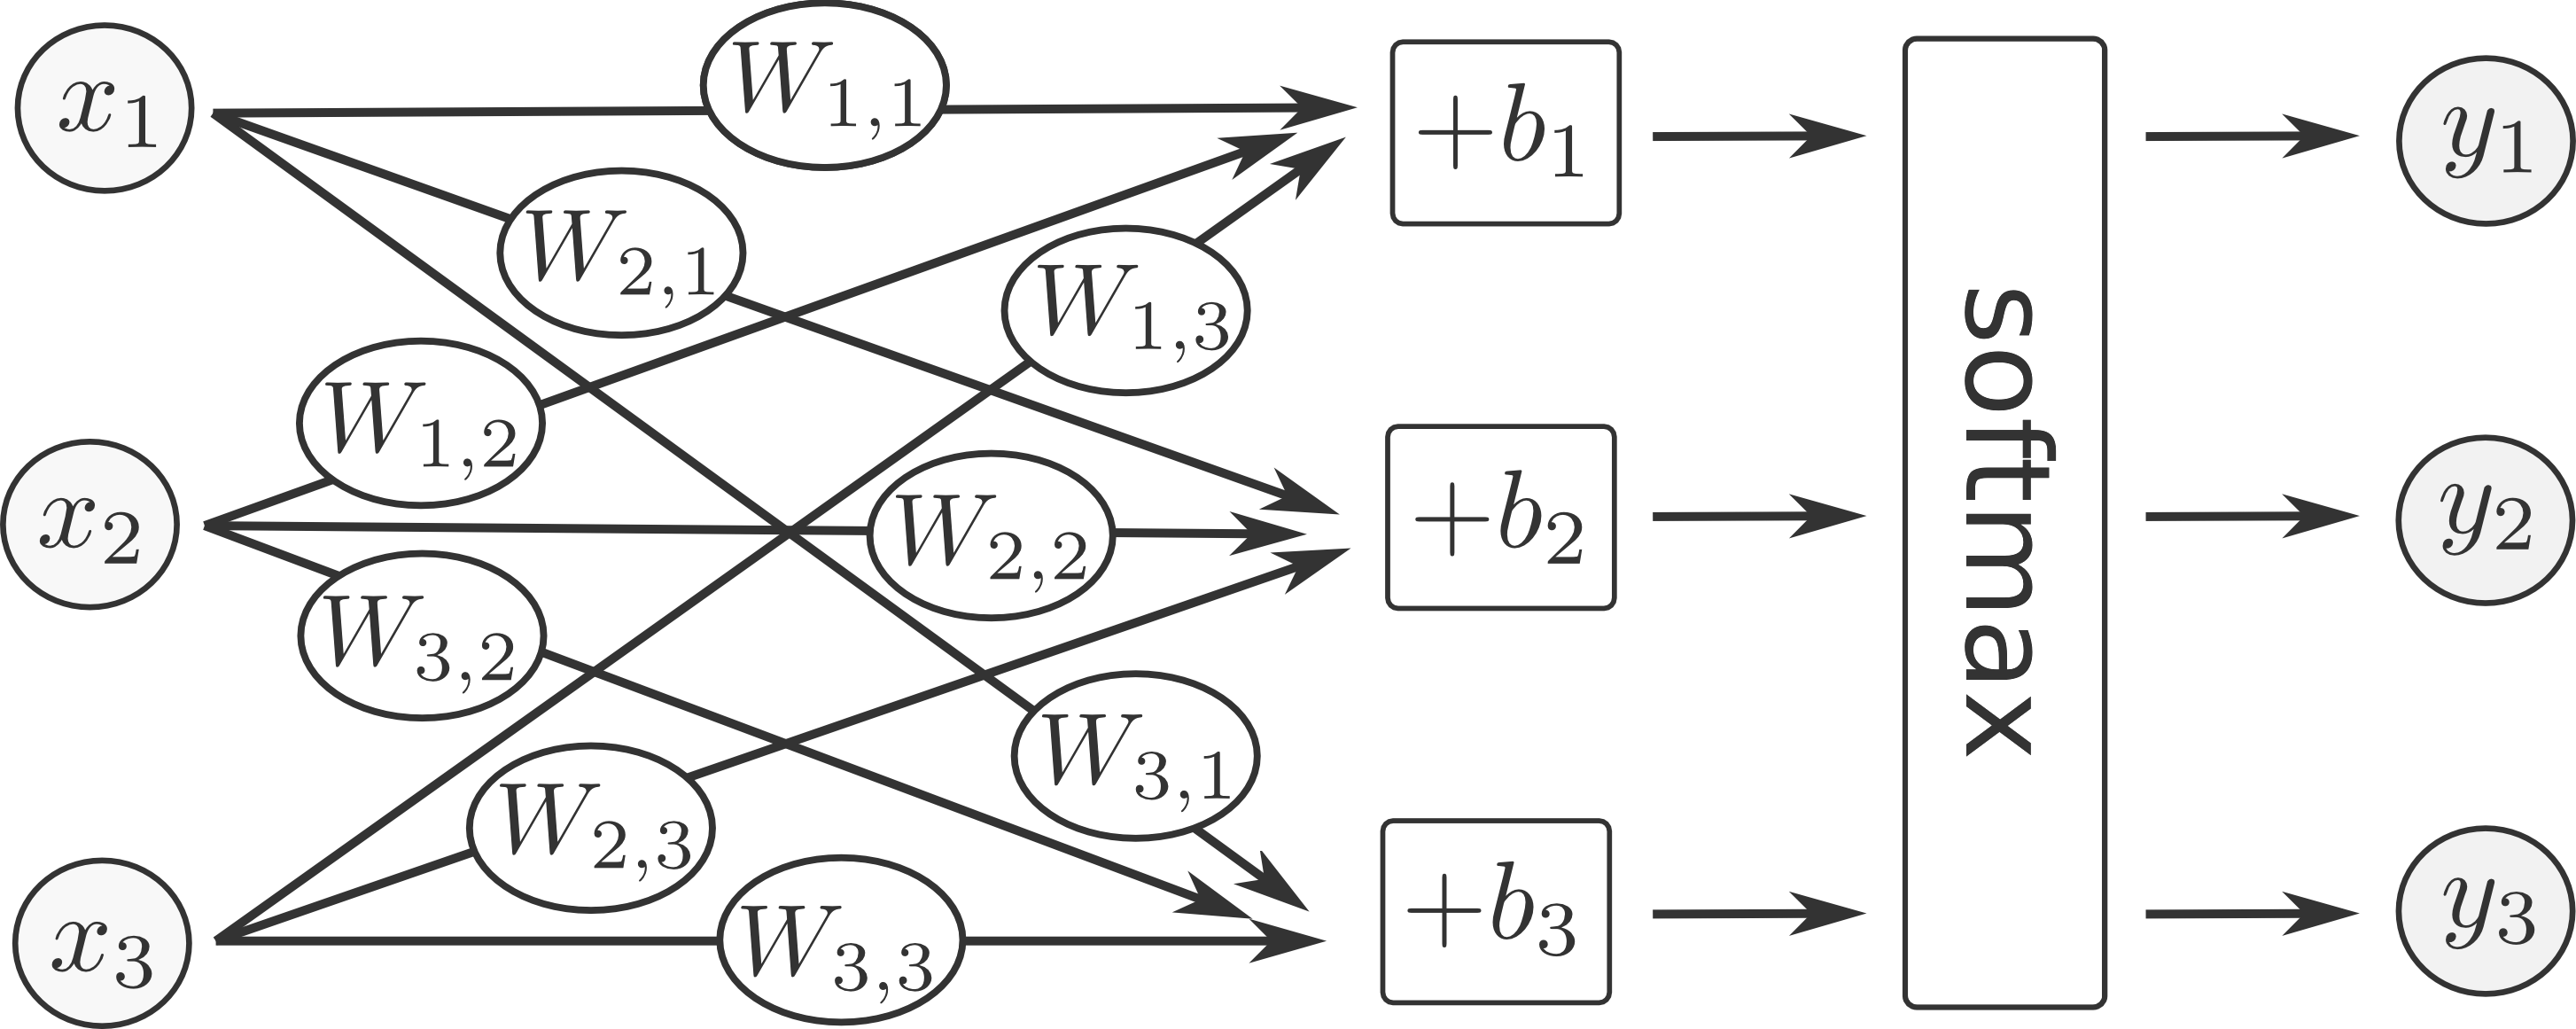
\includegraphics[width=8cm]{images/model-graph.png}
\caption{Simplified representation of model graph \cite{tf}}
\end{figure}

\paragraph{Training} We employ gradient-descent on mini-batches. Early-stopping prevents the model from further learning when performance on the validation split starts decreasing.

\paragraph{Prediction}
TODO

\paragraph{Evaluation}
TODO

\begin{center}
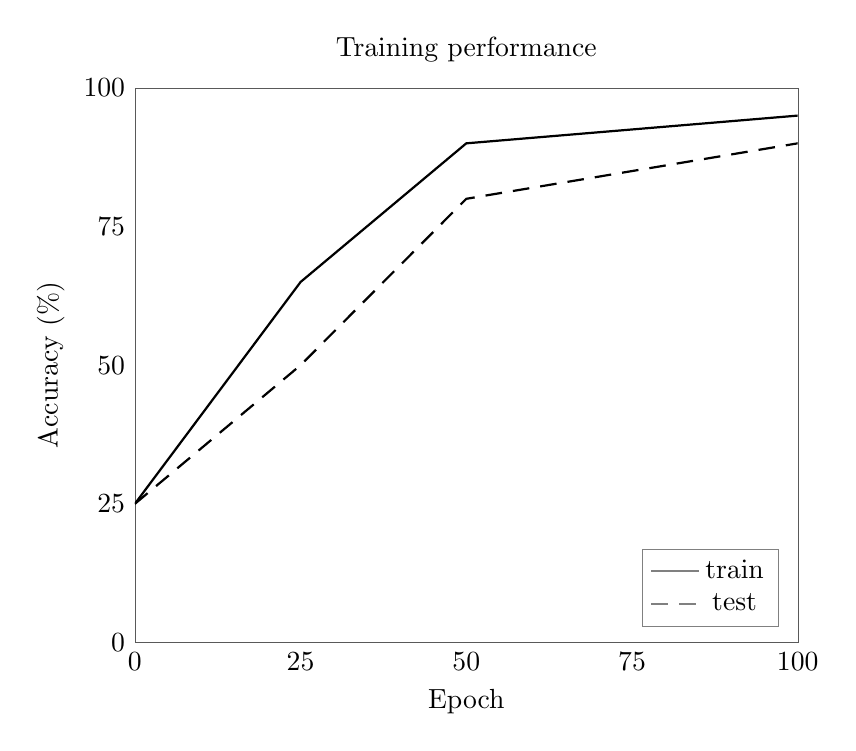
\begin{tikzpicture}
\begin{axis} [
  title={Training performance},
  xlabel={Epoch},
  ylabel={Accuracy (\%)},
  xmin=0, xmax=100,
  ymin=0, ymax=100,
  xtick={0,25,50,75,100},
  ytick={0,25,50,75,100},
  legend pos=south east,
  axis line style={black!65, line width=.1pt}, % thinner frame border
  legend style={draw=black!50, line width=.1pt}, % thinner frame border
  every x tick/.style={white}, % hide x ticks (make them white)
  every y tick/.style={white}, % hide y ticks (make them white)
  every axis plot/.append style={thick},
]

\addplot[]
  coordinates {
  (0,25)(25,65)(50,90)(100,95)
  };
\addplot[dash pattern=on 6pt off 4pt]
  coordinates {
  (0,25)(25,50)(50,80)(100,90)
  };
  
\legend{train, test}
\end{axis}
\end{tikzpicture}
\end{center}



\newpage
\section{Parallelization}
Parallelism is needed in the training phase of the model, as prediction happens instantaneously

TODO: talk about matrix multiplication overhead

TODO: graph of train time vs nr of processors

\begin{center}
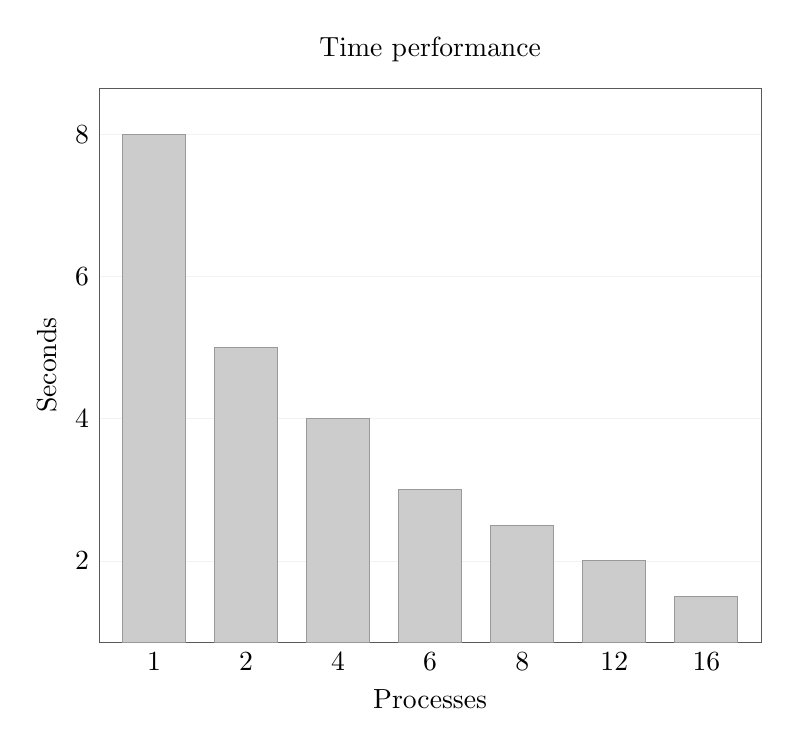
\begin{tikzpicture}
\begin{axis}[
  title={Time performance},
  xlabel=Processes,
  ylabel=Seconds,
  bar width=.8cm,
  axis line style={black!65, line width=.1pt}, % thinner border
  symbolic x coords={1,2,4,6,8,12,16}, % equidistant bars
  every x tick/.style={white}, % hide x ticks (make them white)
  every y tick/.style={line width=.1pt, draw=gray!10}, % y ticks same color as grid
  ymajorgrids=true, % show horizontal grid lines
  grid style={line width=.1pt, draw=gray!10}, % gray grid lines
  ]
  \addplot[ybar, black!40, fill=black!20] coordinates {
      (1,8) 
      (2,5)
      (4,4) 
      (6,3) 
      (8,2.5) 
      (12,2) 
      (16,1.5)    
      };
\end{axis}
\end{tikzpicture}
\end{center}



\newpage
\section{Graphical Interface}
TODO: picture of resizing

TODO: picture of GUI



\newpage
\section{Implementation}
After going through the high-level overview of the project, we now delve into implementation details.

\paragraph{Predictive model} The core of the project is implemented in C++. This includes the neural network training and prediction. Data is maintained in memory using vectors from the standard library.

\paragraph{Graphical Interface} The GUI is implemented as a web page in HTML, with a canvas for the input box.
The drawing is facilitated by the Sketch library \cite{sketch}. Interactivity and picture resizing is done through JavaScript.

\paragraph{Communication Server} The glue between the front-end and the model is a web-server done in Python, using the Flask library \cite{flask}. An array of $784$ pixels is received through from the GUI and is passed to the compiled executable. The output (predicted digit and prediction confidence) is then passed back through AJAX.
\\

The entire source code is available at \url{https://github.com/stefan1niculae/mnist-in-mpi}.

\vspace{\fill} % place references at the bottom
\bibliographystyle{ieeetr}
	\bibliography{references} % expects file "references.bib"
	\addcontentsline{toc}{section}{References}
    
    

\end{document}
